\documentclass[12pt,a4paper]{article}

% Packages
\usepackage[utf8]{inputenc}
\usepackage[T1]{fontenc}
\usepackage{lmodern}
\usepackage[margin=1in, headheight=14pt]{geometry}
\usepackage{graphicx}
\usepackage{hyperref}
\usepackage{enumitem}
\usepackage{booktabs}
\usepackage{longtable}
\usepackage{xcolor}
\usepackage{listings}
\usepackage{fancyhdr}
\usepackage{titlesec}
\usepackage{tocloft}
\usepackage{float}
\usepackage{caption}
\usepackage{parskip}
\usepackage{tikz}
\usetikzlibrary{shapes.geometric, arrows.meta, positioning, fit, backgrounds, calc}

% C4 Diagram Styles
\tikzstyle{person} = [rectangle, rounded corners=8pt, minimum width=2.8cm, minimum height=1.6cm, text centered, draw=blue!70!black, fill=blue!15, font=\small\bfseries, text width=2.6cm]
\tikzstyle{system} = [rectangle, rounded corners=4pt, minimum width=3.2cm, minimum height=1.6cm, text centered, draw=blue!60!black, fill=blue!25, font=\small\bfseries, text width=3cm]
\tikzstyle{externalsys} = [rectangle, rounded corners=4pt, minimum width=3cm, minimum height=1.4cm, text centered, draw=gray!70, fill=gray!15, font=\small\bfseries, text width=2.8cm]
\tikzstyle{container} = [rectangle, rounded corners=4pt, minimum width=2.6cm, minimum height=1.4cm, text centered, draw=blue!50!black, fill=blue!10, font=\scriptsize\bfseries, text width=2.4cm]
\tikzstyle{database} = [cylinder, shape border rotate=90, draw=orange!70!black, fill=orange!10, minimum width=2cm, minimum height=1.2cm, text centered, font=\scriptsize\bfseries, text width=1.8cm, aspect=0.3]
\tikzstyle{infra} = [rectangle, rounded corners=4pt, minimum width=2.2cm, minimum height=1.2cm, text centered, draw=green!50!black, fill=green!8, font=\scriptsize\bfseries, text width=2cm]
\tikzstyle{component} = [rectangle, rounded corners=3pt, minimum width=3cm, minimum height=1cm, text centered, draw=teal!60!black, fill=teal!8, font=\scriptsize\bfseries, text width=2.8cm]
\tikzstyle{arrow} = [-{Stealth[length=2mm]}, thick, draw=gray!70]
\tikzstyle{arrowlabel} = [font=\tiny, fill=white, inner sep=1pt]
\tikzstyle{dashedarrow} = [-{Stealth[length=2mm]}, thick, dashed, draw=gray!60]

% Colors
\definecolor{zewailblue}{RGB}{0,51,102}
\definecolor{linkblue}{RGB}{0,102,204}

% Hyperref setup
\hypersetup{
    colorlinks=true,
    linkcolor=zewailblue,
    urlcolor=linkblue,
    citecolor=zewailblue
}

% Header/Footer
\pagestyle{fancy}
\fancyhf{}
\fancyhead[L]{\small SWAPD 351 -- Software Architecture and Design}
\fancyhead[R]{\small Eventify Platform}
\fancyfoot[C]{\thepage}
\renewcommand{\headrulewidth}{0.4pt}

% Title formatting
\titleformat{\section}{\Large\bfseries\color{zewailblue}}{}{0em}{}[\titlerule]
\titleformat{\subsection}{\large\bfseries\color{zewailblue}}{}{0em}{}

% Code listing style
\lstset{
    basicstyle=\ttfamily\small,
    frame=single,
    breaklines=true,
    backgroundcolor=\color{gray!5}
}

\begin{document}

% ---- TITLE PAGE ----
\begin{titlepage}
\centering
\vspace*{1cm}

{\Huge\bfseries\color{zewailblue} Eventify Platform}\\[0.5cm]
{\Large High-Level System Design Document}\\[0.3cm]
{\large Phase 1 Submission}

\vspace{1.5cm}

{\large\textbf{SWAPD 351 -- Software Architecture and Design}}\\[0.3cm]
{\large Spring 2026}

\vspace{2cm}

{\large\textbf{Team Members}}\\[0.5cm]
\begin{tabular}{l}
Habiba Magdy \\
Basmala Salah \\
Arwa Mohamed \\
Lana Mohamed \\
\end{tabular}

\vspace{2cm}

{\large Zewail City of Science and Technology}\\[0.3cm]
{\large University of Science and Technology}

\vfill
{\small Document Version 1.0 --- \today}
\end{titlepage}

% ---- TABLE OF CONTENTS ----
\tableofcontents
\newpage

% ======================================================================
% SECTION 1: REQUIREMENTS SPECIFICATION
% ======================================================================
\section{Requirements Specification Document}

\subsection{Project Overview}

Eventify is an event management platform built on a microservices architecture. The system allows users to create, browse, and RSVP to events, communicate through real-time chat, and view event analytics on a live dashboard. The platform uses OAuth2 (Google) for authentication, an API Gateway for request routing, and asynchronous messaging for inter-service communication.

\subsection{Functional Requirements}

\begin{enumerate}[label=\textbf{FR-\arabic*}]
    \item \textbf{User Registration and Authentication}: Users shall be able to register and log in using Google OAuth2. The system shall issue JWT tokens upon successful authentication.
    \item \textbf{Event Creation}: Authenticated users shall be able to create events with a title, description, date, time, location, and maximum capacity.
    \item \textbf{Event Browsing}: Users shall be able to browse and search for events by date, category, or keyword.
    \item \textbf{Event RSVP}: Authenticated users shall be able to RSVP to events. The system shall enforce capacity limits.
    \item \textbf{Event Update and Deletion}: Event creators shall be able to update or delete their own events.
    \item \textbf{Real-Time Chat}: Users who have RSVP'd to an event shall be able to send and receive messages in an event-specific chat room.
    \item \textbf{Notifications}: The system shall send notifications when a user RSVPs, when an event is updated, or when a new chat message is posted.
    \item \textbf{Dashboard}: An analytics dashboard shall display real-time data including total events, total RSVPs, trending events, and user activity metrics.
    \item \textbf{User Profile}: Users shall be able to view and edit their profile information and see their RSVP history.
\end{enumerate}

\subsection{Non-Functional Requirements (Quality Attributes)}

\begin{enumerate}[label=\textbf{NFR-\arabic*}]
    \item \textbf{Scalability}: The system shall scale horizontally. Each microservice shall be independently deployable and scalable. The database shall support sharding for high-volume data.
    \item \textbf{Performance}: API response times shall be under 200ms for read operations under normal load. The dashboard shall refresh data within 2 seconds.
    \item \textbf{Availability}: The system shall target 99.9\% uptime. Circuit breakers shall prevent cascading failures across services.
    \item \textbf{Security}: All API endpoints shall require valid JWT tokens. Data in transit shall be encrypted using TLS. OAuth2 tokens shall be short-lived with refresh capability.
    \item \textbf{Resilience}: The system shall implement circuit breakers on all inter-service calls and retry logic with exponential backoff for transient failures.
    \item \textbf{Observability}: Centralized logging (OpenSearch), application metrics (Prometheus + Grafana), and distributed tracing shall be implemented.
    \item \textbf{Maintainability}: Each service shall follow clean architecture principles. Services shall be containerized using Docker and orchestrated using Docker Compose.
\end{enumerate}

\subsection{User Stories / Use Cases}

\begin{longtable}{p{2cm}p{4cm}p{7cm}}
\toprule
\textbf{ID} & \textbf{Title} & \textbf{Description} \\
\midrule
\endhead
US-01 & User Login & As a user, I want to log in with my Google account so that I do not need to create a separate password. \\
\midrule
US-02 & Create Event & As an authenticated user, I want to create an event with details so that others can discover and join it. \\
\midrule
US-03 & Browse Events & As a user, I want to search and filter events by date or category so that I can find relevant events quickly. \\
\midrule
US-04 & RSVP to Event & As an authenticated user, I want to RSVP to an event so that I can reserve my spot. \\
\midrule
US-05 & Cancel RSVP & As a user, I want to cancel my RSVP if my plans change. \\
\midrule
US-06 & Event Chat & As an event attendee, I want to chat with other attendees in real-time so that we can coordinate. \\
\midrule
US-07 & Receive Notifications & As a user, I want to receive notifications about event updates and new messages. \\
\midrule
US-08 & View Dashboard & As a user, I want to see a dashboard with trending events and activity metrics. \\
\midrule
US-09 & Edit Profile & As a user, I want to update my profile information and view my event history. \\
\midrule
US-10 & Delete Event & As an event creator, I want to delete my event if it is cancelled. \\
\bottomrule
\end{longtable}

\subsection{Architectural Drivers}

The following quality attributes drive the architectural decisions:

\begin{itemize}
    \item \textbf{Scalability}: Independent scaling of services under varying load (e.g., event browsing may spike during weekends). This drives the choice of microservices over a monolithic architecture.
    \item \textbf{Resilience}: The system must tolerate individual service failures without full system downtime. This drives the adoption of circuit breakers, retries, and asynchronous messaging.
    \item \textbf{Security}: Sensitive user data and authentication tokens must be protected. This drives the choice of OAuth2 with JWT and TLS encryption.
    \item \textbf{Performance}: Read-heavy workloads on event browsing and dashboard require caching. This drives the adoption of Redis for caching and session management.
    \item \textbf{Observability}: In a distributed system, tracing requests across services is critical for debugging. This drives centralized logging with OpenSearch and monitoring with Prometheus/Grafana.
\end{itemize}

\newpage

% ======================================================================
% SECTION 2: C4 MODEL DIAGRAMS
% ======================================================================
\section{C4 Model Diagrams}

This section presents the system architecture using the C4 model at three levels of abstraction. Full-resolution diagrams are provided alongside this document in PNG/SVG format.

\subsection{Level 1: Context Diagram}

The Context Diagram shows Eventify as a single system, its users, and external dependencies.

\begin{figure}[H]
\centering
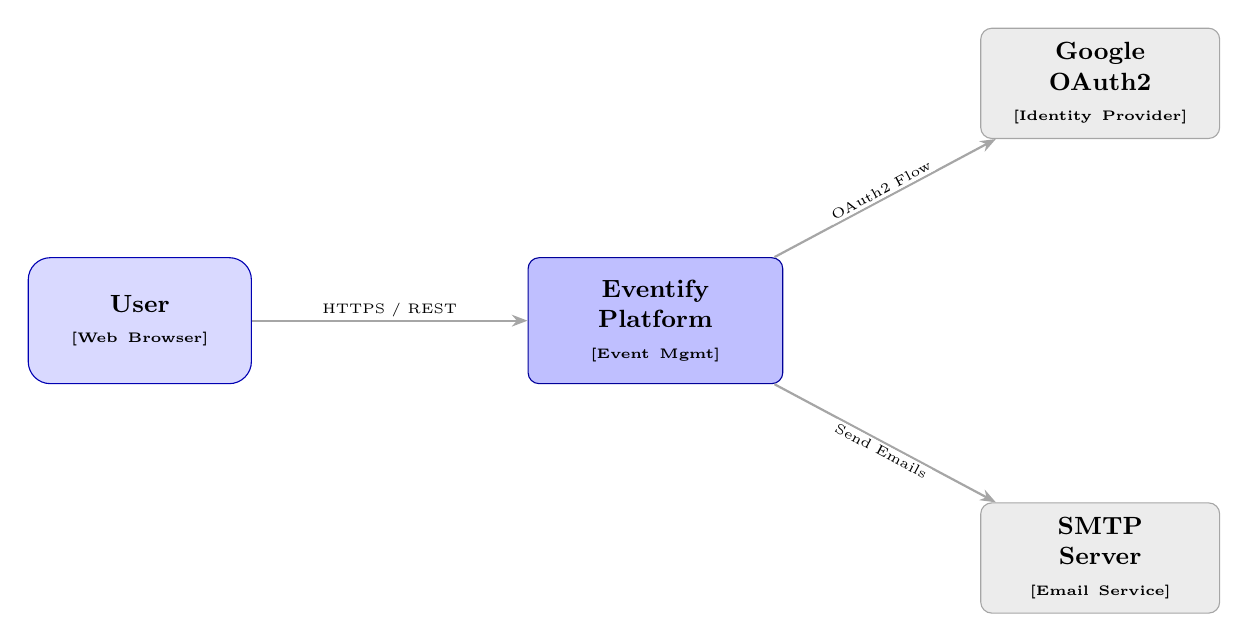
\begin{tikzpicture}[node distance=1.8cm]
    % Nodes
    \node[person] (user) {User\\{\tiny[Web Browser]}};
    \node[system, right=3.5cm of user] (eventify) {Eventify\\Platform\\{\tiny[Event Mgmt]}};
    \node[externalsys, above right=1.5cm and 2.5cm of eventify] (google) {Google\\OAuth2\\{\tiny[Identity Provider]}};
    \node[externalsys, below right=1.5cm and 2.5cm of eventify] (smtp) {SMTP\\Server\\{\tiny[Email Service]}};

    % Arrows
    \draw[arrow] (user) -- node[arrowlabel, above] {HTTPS / REST} (eventify);
    \draw[arrow] (eventify) -- node[arrowlabel, above, sloped] {OAuth2 Flow} (google);
    \draw[arrow] (eventify) -- node[arrowlabel, below, sloped] {Send Emails} (smtp);
\end{tikzpicture}
\caption{Level 1 -- System Context Diagram}
\end{figure}

\textbf{Description}: Users interact with the Eventify Platform through a web browser over HTTPS. The system depends on Google OAuth2 for authentication and an SMTP server for sending email notifications.

\subsection{Level 2: Container Diagram}

The Container Diagram breaks Eventify into its constituent containers (services, databases, caches).

\begin{figure}[H]
\centering
\resizebox{0.98\textwidth}{!}{%
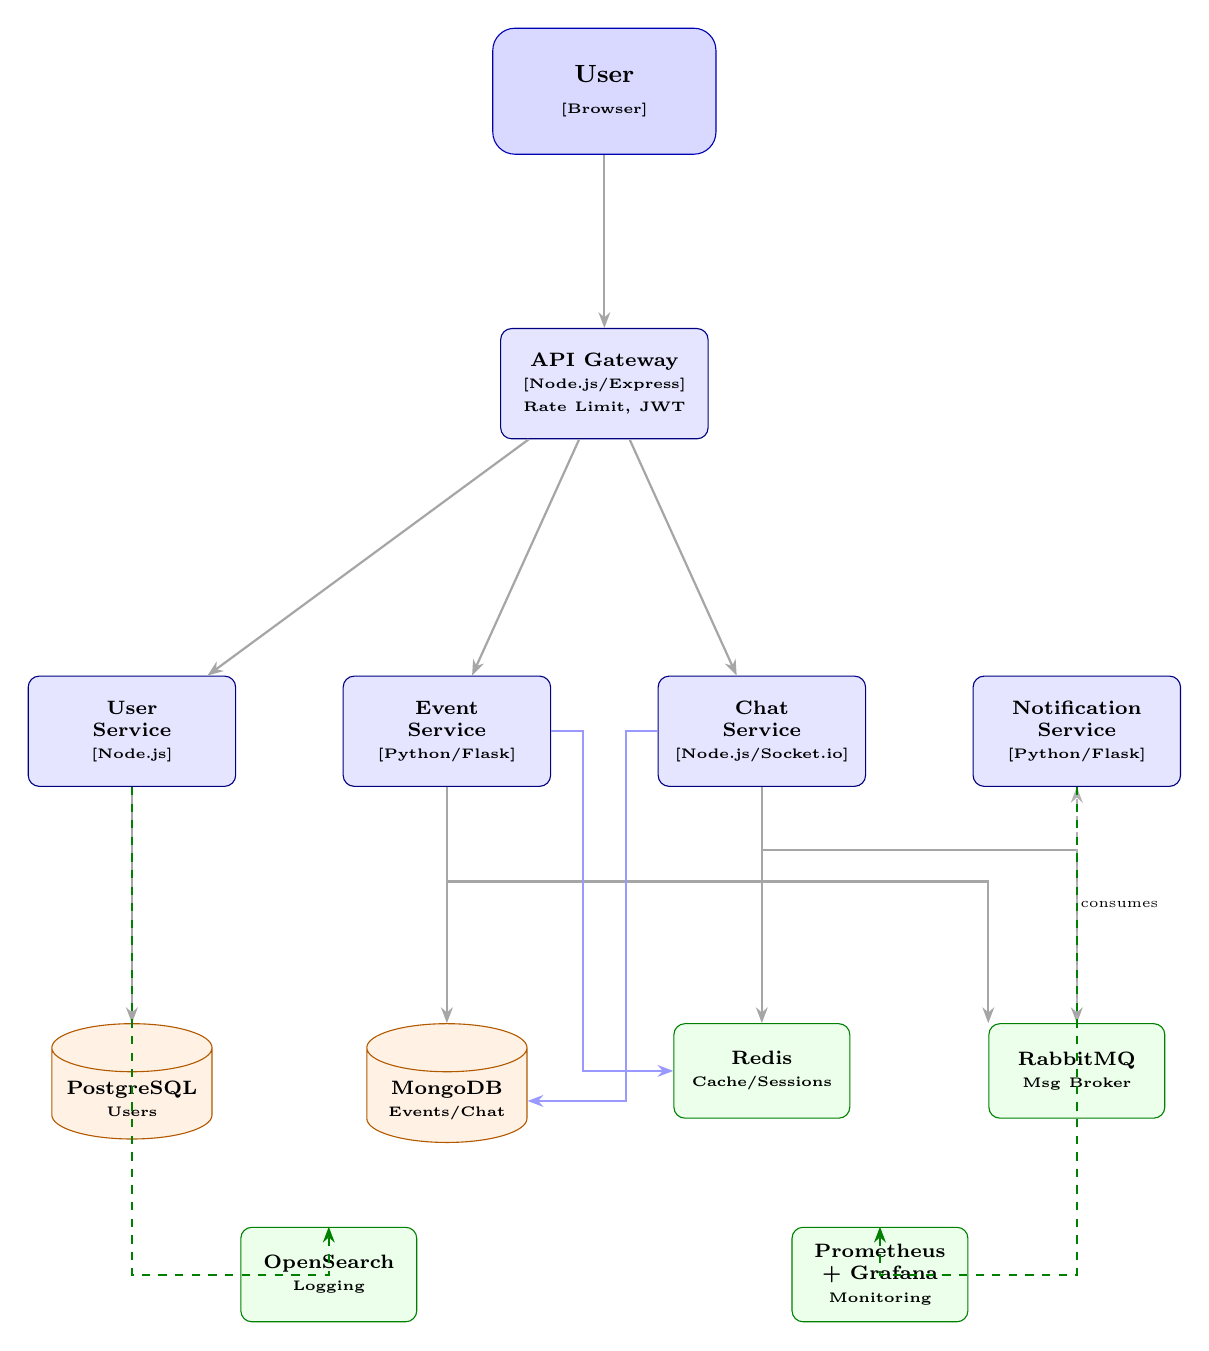
\begin{tikzpicture}[node distance=2cm and 1.5cm]
    % === ROW 1: User ===
    \node[person] (user) {User\\{\tiny[Browser]}};

    % === ROW 2: API Gateway ===
    \node[container, below=2.2cm of user] (gw) {API Gateway\\{\tiny[Node.js/Express]}\\{\tiny Rate Limit, JWT}};

    % === ROW 3: Microservices (evenly spaced, wide) ===
    \node[container, below=3cm of gw, xshift=-6cm] (usersvc) {User\\Service\\{\tiny[Node.js]}};
    \node[container, below=3cm of gw, xshift=-2cm] (eventsvc) {Event\\Service\\{\tiny[Python/Flask]}};
    \node[container, below=3cm of gw, xshift=2cm] (chatsvc) {Chat\\Service\\{\tiny[Node.js/Socket.io]}};
    \node[container, below=3cm of gw, xshift=6cm] (notifsvc) {Notification\\Service\\{\tiny[Python/Flask]}};

    % === ROW 4: Data Stores (each directly below its service) ===
    \node[database, below=3cm of usersvc] (pg) {PostgreSQL\\{\tiny Users}};
    \node[database, below=3cm of eventsvc] (mongo) {MongoDB\\{\tiny Events/Chat}};
    \node[infra, below=3cm of chatsvc] (redis) {Redis\\{\tiny Cache/Sessions}};
    \node[infra, below=3cm of notifsvc] (rabbit) {RabbitMQ\\{\tiny Msg Broker}};

    % === ROW 5: Observability (centered, separate row far below) ===
    \node[infra, below=10cm of gw, xshift=-3.5cm] (opensearch) {OpenSearch\\{\tiny Logging}};
    \node[infra, below=10cm of gw, xshift=3.5cm] (promgraf) {Prometheus\\+ Grafana\\{\tiny Monitoring}};

    % ===== ARROWS =====
    % User -> Gateway
    \draw[arrow] (user) -- (gw);

    % Gateway -> Services (only 3 shown; notification is consumer-only)
    \draw[arrow] (gw) -- (usersvc);
    \draw[arrow] (gw) -- (eventsvc);
    \draw[arrow] (gw) -- (chatsvc);

    % Each service -> its own DB (straight down, no crossing)
    \draw[arrow] (usersvc) -- (pg);
    \draw[arrow] (eventsvc) -- (mongo);
    \draw[arrow] (chatsvc) -- (redis);

    % Event Service -> RabbitMQ (clean right-angle)
    \draw[arrow] (eventsvc.south) -- ++(0,-1.2) -| (rabbit.north west);

    % Chat Service -> RabbitMQ (clean right-angle)
    \draw[arrow] (chatsvc.south) -- ++(0,-0.8) -| (rabbit.north);

    % Notification Service consumes from RabbitMQ (dashed upward)
    \draw[dashedarrow] (rabbit) -- node[arrowlabel, right] {\tiny consumes} (notifsvc);

    % Event Service also uses Redis (right-angle, goes right)
    \draw[arrow, draw=blue!40] (eventsvc.east) -- ++(0.4,0) |- (redis.west);

    % Chat Service also stores in MongoDB
    \draw[arrow, draw=blue!40] (chatsvc.west) -- ++(-0.4,0) |- (mongo.east);

    % Observability (simple dotted lines going straight down, no routing)
    \draw[dashedarrow, draw=green!50!black] (usersvc.south) -- ++(0,-6.2) -| (opensearch.north);
    \draw[dashedarrow, draw=green!50!black] (notifsvc.south) -- ++(0,-6.2) -| (promgraf.north);
\end{tikzpicture}
}%
\caption{Level 2 -- Container Diagram}
\end{figure}

\textbf{Container Descriptions}:
\begin{itemize}
    \item \textbf{API Gateway (Node.js/Express)}: Entry point for all client requests. Routes requests to appropriate services, handles rate limiting, and validates JWT tokens.
    \item \textbf{User Service (Node.js/Express)}: Manages user registration, OAuth2 authentication with Google, profile management, and JWT token issuance.
    \item \textbf{Event Service (Python/Flask)}: Handles CRUD operations for events and RSVPs. Stores data in MongoDB. Publishes events to RabbitMQ on state changes.
    \item \textbf{Notification Service (Python/Flask)}: Consumes messages from RabbitMQ and sends notifications via WebSocket push and email (SMTP).
    \item \textbf{Chat Service (Node.js/Socket.io)}: Provides real-time messaging using WebSockets. Stores chat history in MongoDB.
    \item \textbf{PostgreSQL}: Relational database for user data and authentication records. Supports sharding through Citus extension.
    \item \textbf{MongoDB}: Document database for events, RSVPs, and chat messages. Supports horizontal scaling via sharding.
    \item \textbf{Redis}: In-memory store for session management, caching frequently accessed event data, and rate limiting counters.
    \item \textbf{RabbitMQ}: Message broker for asynchronous communication between services (event updates, notifications).
    \item \textbf{OpenSearch}: Centralized log aggregation and search for all services.
    \item \textbf{Prometheus + Grafana}: Metrics collection and visualization for monitoring application and host metrics.
\end{itemize}

\subsection{Level 3: Component Diagram -- Event Service}

The Component Diagram shows the internal structure of the Event Service.

\begin{figure}[H]
\centering
\resizebox{0.95\textwidth}{!}{%
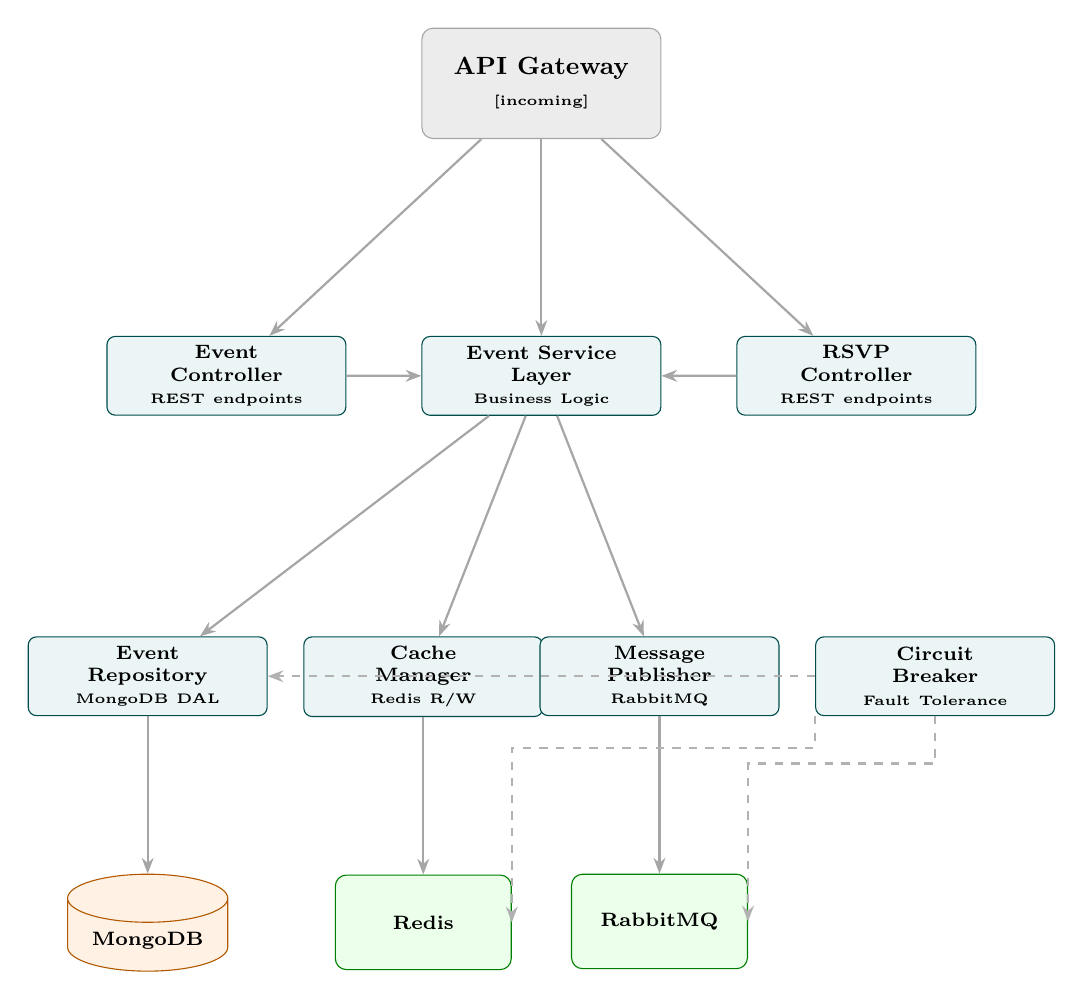
\begin{tikzpicture}[node distance=2cm and 2.5cm]
    % External entry
    \node[externalsys, minimum width=3cm] (apigw) {API Gateway\\{\tiny[incoming]}};

    % Controllers (Row 2, spread wide)
    \node[component, below=2.5cm of apigw, xshift=-4cm] (eventctrl) {Event\\Controller\\{\tiny REST endpoints}};
    \node[component, below=2.5cm of apigw] (svclay) {Event Service\\Layer\\{\tiny Business Logic}};
    \node[component, below=2.5cm of apigw, xshift=4cm] (rsvpctrl) {RSVP\\Controller\\{\tiny REST endpoints}};

    % Bottom row (Row 3, spread wide)
    \node[component, below=2.8cm of svclay, xshift=-5cm] (repo) {Event\\Repository\\{\tiny MongoDB DAL}};
    \node[component, below=2.8cm of svclay, xshift=-1.5cm] (cache) {Cache\\Manager\\{\tiny Redis R/W}};
    \node[component, below=2.8cm of svclay, xshift=1.5cm] (pub) {Message\\Publisher\\{\tiny RabbitMQ}};
    \node[component, below=2.8cm of svclay, xshift=5cm] (cb) {Circuit\\Breaker\\{\tiny Fault Tolerance}};

    % External stores (Row 4)
    \node[database, below=2cm of repo] (mongodb) {MongoDB};
    \node[infra, below=2cm of cache] (redisdb) {Redis};
    \node[infra, below=2cm of pub] (rabbitmq) {RabbitMQ};

    % Arrows
    \draw[arrow] (apigw) -- (eventctrl);
    \draw[arrow] (apigw) -- (svclay);
    \draw[arrow] (apigw) -- (rsvpctrl);
    \draw[arrow] (eventctrl) -- (svclay);
    \draw[arrow] (rsvpctrl) -- (svclay);
    \draw[arrow] (svclay) -- (repo);
    \draw[arrow] (svclay) -- (cache);
    \draw[arrow] (svclay) -- (pub);
    \draw[arrow] (repo) -- (mongodb);
    \draw[arrow] (cache) -- (redisdb);
    \draw[arrow] (pub) -- (rabbitmq);

    % Circuit breaker wraps (dashed, routed cleanly)
    \draw[dashedarrow] (cb.south) -- ++(0,-0.6) -| (rabbitmq.east);
    \draw[dashedarrow] (cb.west) -- ++(-0.5,0) |- (repo.east);
    \draw[dashedarrow] (cb.south west) -- ++(0,-0.4) -| (redisdb.east);
\end{tikzpicture}
}%
\caption{Level 3 -- Component Diagram of Event Service}
\end{figure}

\textbf{Interaction Flow}:
\begin{enumerate}
    \item A request arrives at the Event Controller via the API Gateway.
    \item The Controller delegates to the Event Service Layer for business logic.
    \item The Service Layer checks Redis cache (via Cache Manager) before querying MongoDB (via Event Repository).
    \item On write operations, the Message Publisher sends an event to RabbitMQ to notify other services.
    \item All external calls (Redis, RabbitMQ, MongoDB) are wrapped with Circuit Breakers.
\end{enumerate}

\newpage

% ======================================================================
% SECTION 3: ARCHITECTURE DECISION RECORDS
% ======================================================================
\section{Architecture Decision Records (ADRs)}

% ADR-001: Microservices Architecture
\subsection{ADR-001: Adoption of Microservices Architecture}

\begin{tabular}{p{3cm}p{10cm}}
\textbf{Status} & Accepted \\
\textbf{Date} & 2026-03-15 \\
\textbf{Decision} & Adopt a microservices architecture over a monolithic architecture. \\
\end{tabular}

\textbf{Context}: The Eventify platform comprises distinct domains: user management, event management, real-time chat, and notifications. These domains have different scaling characteristics. Event browsing may experience high read traffic, while chat requires persistent WebSocket connections. A monolithic application would force all domains to scale together, wasting resources.

\textbf{Decision}: Decompose the system into five independently deployable microservices: API Gateway, User Service, Event Service, Chat Service, and Notification Service. Each service owns its data and communicates via REST (synchronous) or RabbitMQ (asynchronous).

\textbf{Consequences}:
\begin{itemize}
    \item \textit{Positive}: Independent scaling, independent deployment, technology flexibility per service, fault isolation.
    \item \textit{Negative}: Increased operational complexity, network latency between services, eventual consistency challenges, need for distributed tracing.
\end{itemize}

\textbf{Alternatives Considered}:
\begin{itemize}
    \item Monolithic architecture --- simpler to develop initially but does not meet scalability and independent deployment requirements.
    \item Service-oriented architecture (SOA) --- heavier governance and shared data layer; microservices provide better autonomy.
\end{itemize}

% ADR-002: Database Selection
\subsection{ADR-002: Database Selection -- PostgreSQL and MongoDB}

\begin{tabular}{p{3cm}p{10cm}}
\textbf{Status} & Accepted \\
\textbf{Date} & 2026-03-15 \\
\textbf{Decision} & Use PostgreSQL for user data and MongoDB for event/chat data. \\
\end{tabular}

\textbf{Context}: The system handles two fundamentally different data patterns. User data (accounts, credentials, OAuth tokens) is relational, requires strong consistency, and benefits from ACID transactions. Event data (events with varying attributes, RSVPs, chat messages) is document-oriented, with flexible schemas and high write throughput requirements.

\textbf{Decision}: Adopt a polyglot persistence strategy:
\begin{itemize}
    \item \textbf{PostgreSQL} for the User Service: stores user profiles, OAuth tokens, and session metadata. Supports sharding via the Citus extension for horizontal scaling.
    \item \textbf{MongoDB} for the Event Service and Chat Service: stores events, RSVPs, and chat messages. MongoDB's document model naturally maps to event objects with nested attendee lists. Native sharding support enables horizontal scaling by event ID or date range.
\end{itemize}

\textbf{Consequences}:
\begin{itemize}
    \item \textit{Positive}: Each database is optimized for its workload. PostgreSQL guarantees consistency for user operations. MongoDB handles high-throughput writes for chat and flexible event schemas.
    \item \textit{Negative}: Operational overhead of managing two database technologies. Cross-database joins are not possible; data must be denormalized or fetched via API calls.
\end{itemize}

\textbf{Sharding Considerations}:
\begin{itemize}
    \item PostgreSQL: Shard by user ID using Citus distributed tables.
    \item MongoDB: Shard events collection by \texttt{event\_id} (hashed) for even distribution. Shard chat messages by \texttt{event\_id} to co-locate messages for the same event.
\end{itemize}

% ADR-003: Authentication Method
\subsection{ADR-003: OAuth2 via Google with JWT Tokens}

\begin{tabular}{p{3cm}p{10cm}}
\textbf{Status} & Accepted \\
\textbf{Date} & 2026-03-15 \\
\textbf{Decision} & Use Google OAuth2 for user authentication and JWT tokens for session management. \\
\end{tabular}

\textbf{Context}: The project requires token-based authentication with OAuth2 via Google as the primary provider. In a microservices architecture, session state must be shareable across services without a centralized session store bottleneck.

\textbf{Decision}: Implement the OAuth2 Authorization Code flow with Google as the identity provider. Upon successful authentication, the User Service issues a signed JWT containing the user's ID and roles. Subsequent requests include this JWT in the Authorization header. The API Gateway validates the JWT signature before routing requests to backend services.

\textbf{Token Strategy}:
\begin{itemize}
    \item Access Token: JWT with 15-minute expiry, signed with RS256.
    \item Refresh Token: Opaque token stored in Redis with 7-day expiry.
    \item Token refresh is handled by the User Service via the \texttt{/api/auth/refresh} endpoint.
\end{itemize}

\textbf{Consequences}:
\begin{itemize}
    \item \textit{Positive}: Stateless authentication at the API Gateway (no database lookup per request). Users benefit from Google's security infrastructure. JWTs are self-contained and can be verified by any service.
    \item \textit{Negative}: JWT revocation is not immediate (must wait for expiry or maintain a blacklist in Redis). Dependency on Google's OAuth2 service availability.
\end{itemize}

% ADR-004: Message Broker Selection
\subsection{ADR-004: RabbitMQ as Message Broker}

\begin{tabular}{p{3cm}p{10cm}}
\textbf{Status} & Accepted \\
\textbf{Date} & 2026-03-15 \\
\textbf{Decision} & Use RabbitMQ for asynchronous inter-service communication. \\
\end{tabular}

\textbf{Context}: The Event Service needs to notify the Notification Service when events are created, updated, or when users RSVP. Similarly, the Chat Service triggers notification alerts. These operations are side-effects and should not block the primary request-response cycle.

\textbf{Decision}: Adopt RabbitMQ with durable queues and topic exchanges. Producers publish messages to exchanges, and consumers bind queues to receive specific message types.

\textbf{Queue Design}:
\begin{itemize}
    \item Exchange: \texttt{eventify.events} (topic exchange)
    \item Routing keys: \texttt{event.created}, \texttt{event.updated}, \texttt{event.deleted}, \texttt{rsvp.created}, \texttt{rsvp.cancelled}, \texttt{chat.message}
    \item Consumer queues: \texttt{notification-queue} (binds to all routing keys)
\end{itemize}

\textbf{Consequences}:
\begin{itemize}
    \item \textit{Positive}: Decouples producers from consumers. Durable queues ensure message delivery even if a consumer is temporarily down. Topic-based routing allows flexible message filtering.
    \item \textit{Negative}: Adds infrastructure complexity. Message ordering is guaranteed only within a single queue. Requires monitoring for queue depth and consumer lag.
\end{itemize}

\textbf{Alternatives Considered}:
\begin{itemize}
    \item Apache Kafka --- better for high-throughput event streaming, but overkill for our notification use case. RabbitMQ's simpler routing model is sufficient.
    \item Redis Pub/Sub --- does not persist messages if the subscriber is offline. Not suitable for reliable notification delivery.
\end{itemize}

% ADR-005: Redis for Caching and Session Management
\subsection{ADR-005: Redis for Caching and Session Management}

\begin{tabular}{p{3cm}p{10cm}}
\textbf{Status} & Accepted \\
\textbf{Date} & 2026-03-15 \\
\textbf{Decision} & Use Redis as the in-memory data store for caching and session management. \\
\end{tabular}

\textbf{Context}: The system requires fast access to frequently read data (event listings, user sessions) and a shared session store accessible by multiple service instances. Read-heavy operations like event browsing benefit from caching to reduce database load and improve response times.

\textbf{Decision}: Deploy a Redis instance shared across services for:
\begin{itemize}
    \item \textbf{Caching}: Cache popular event listings and event details with a TTL of 5 minutes. Cache invalidation occurs on event updates via a write-through strategy.
    \item \textbf{Session Management}: Store refresh tokens and active session metadata. Sessions expire after 7 days of inactivity.
    \item \textbf{Rate Limiting}: Store request counters per user with a sliding window of 1 minute.
\end{itemize}

\textbf{Consequences}:
\begin{itemize}
    \item \textit{Positive}: Sub-millisecond read latency. Reduces load on PostgreSQL and MongoDB. Atomic operations for rate limiting counters.
    \item \textit{Negative}: Additional infrastructure component. Data loss on restart if persistence is not configured (mitigated by using Redis with AOF persistence). Cache invalidation must be carefully managed to avoid stale data.
\end{itemize}

% ADR-006: Multi-Language Microservices
\subsection{ADR-006: Multi-Language Service Implementation}

\begin{tabular}{p{3cm}p{10cm}}
\textbf{Status} & Accepted \\
\textbf{Date} & 2026-03-15 \\
\textbf{Decision} & Implement services in both Node.js and Python based on domain requirements. \\
\end{tabular}

\textbf{Context}: The project description states that not all microservices need to be implemented in the same programming language, and the language choices should be justified in the ADR. Different services have different runtime characteristics that favor different languages.

\textbf{Decision}:
\begin{itemize}
    \item \textbf{Node.js (JavaScript)}: Used for the API Gateway, User Service, and Chat Service. Node.js excels at I/O-bound operations and has native support for WebSockets via Socket.io. Passport.js provides a mature OAuth2 integration for the User Service. The event-driven, non-blocking architecture is ideal for handling many concurrent WebSocket connections in the Chat Service.
    \item \textbf{Python (Flask)}: Used for the Event Service and Notification Service. Python offers concise syntax for CRUD operations and data validation with libraries like Marshmallow. The team has strong familiarity with Python. Flask's simplicity allows rapid development of RESTful APIs without unnecessary abstraction.
\end{itemize}

\textbf{Consequences}:
\begin{itemize}
    \item \textit{Positive}: Each service uses the language best suited to its workload. Team members can work in their strongest language. Demonstrates polyglot microservices as required.
    \item \textit{Negative}: Requires maintaining build tooling and dependency management for two ecosystems (npm and pip). Shared libraries or utilities cannot be easily reused across languages.
\end{itemize}


\newpage

% ======================================================================
% SECTION 4: API SPECIFICATIONS
% ======================================================================
\section{API Specifications}

The full OpenAPI 3.0 specifications for both APIs are provided in the \texttt{api-specs/} directory. Below is a summary of the endpoints.

\subsection{Synchronous vs.\ Asynchronous Communication}

\textbf{Synchronous (REST over HTTP)}:
\begin{itemize}
    \item Client $\rightarrow$ API Gateway $\rightarrow$ User Service (login, profile)
    \item Client $\rightarrow$ API Gateway $\rightarrow$ Event Service (CRUD, RSVP)
    \item These are request-response interactions where the client expects an immediate response.
\end{itemize}

\textbf{Asynchronous (RabbitMQ Message Broker)}:
\begin{itemize}
    \item Event Service $\rightarrow$ RabbitMQ $\rightarrow$ Notification Service (event updates, RSVP confirmations)
    \item Chat Service $\rightarrow$ RabbitMQ $\rightarrow$ Notification Service (new message alerts)
    \item These are fire-and-forget interactions. The producer does not wait for the consumer to process the message.
\end{itemize}

\textbf{Justification}: Synchronous communication is used for user-facing operations that require immediate feedback (e.g., creating an event and receiving a confirmation). Asynchronous communication is used for side-effects like notifications, where the user does not need to wait for the notification to be delivered before receiving a response to their original request. This decouples services and improves resilience --- if the Notification Service is down, event creation still succeeds, and notifications are delivered once the service recovers (messages are persisted in RabbitMQ).

\subsection{Event Service API -- Summary}

\begin{longtable}{@{}p{1.8cm}p{5.5cm}p{6.5cm}@{}}
\toprule
\textbf{Method} & \textbf{Endpoint} & \textbf{Description} \\
\midrule
\endhead
GET & \texttt{/api/events} & List all events (pagination, filtering) \\
\midrule
POST & \texttt{/api/events} & Create a new event (requires auth) \\
\midrule
GET & \texttt{/api/events/\{id\}} & Get event details by ID \\
\midrule
PUT & \texttt{/api/events/\{id\}} & Update an event (creator only) \\
\midrule
DELETE & \texttt{/api/events/\{id\}} & Delete an event (creator only) \\
\midrule
POST & \texttt{/api/events/\{id\}/rsvp} & RSVP to an event (requires auth) \\
\midrule
DELETE & \texttt{/api/events/\{id\}/rsvp} & Cancel RSVP (requires auth) \\
\midrule
GET & \texttt{/api/events/\{id\}/attendees} & List attendees of an event \\
\bottomrule
\end{longtable}

\subsection{User Service API -- Summary}

\begin{longtable}{@{}p{1.8cm}p{5.5cm}p{6.5cm}@{}}
\toprule
\textbf{Method} & \textbf{Endpoint} & \textbf{Description} \\
\midrule
\endhead
GET & \texttt{/api/auth/google} & Initiates Google OAuth2 login flow \\
\midrule
GET & \texttt{/api/auth/google/callback} & OAuth2 callback, issues JWT \\
\midrule
POST & \texttt{/api/auth/refresh} & Refresh an expired JWT token \\
\midrule
GET & \texttt{/api/users/me} & Get current user profile \\
\midrule
PUT & \texttt{/api/users/me} & Update current user profile \\
\midrule
GET & \texttt{/api/users/\{id\}} & Get user profile by ID \\
\bottomrule
\end{longtable}

\newpage

% ======================================================================
% SECTION 5: RESILIENCE STRATEGIES
% ======================================================================
\section{Resilience Strategies}

\subsection{Circuit Breaker Pattern}

All inter-service HTTP calls are protected by circuit breakers. When a downstream service (e.g., the Notification Service) fails consecutively, the circuit opens and immediately returns a fallback response instead of waiting for a timeout.

\textbf{Implementation}: The circuit breaker has three states:
\begin{itemize}
    \item \textbf{Closed}: Requests pass through normally. Failures are counted.
    \item \textbf{Open}: After a threshold of failures (e.g., 5 failures in 30 seconds), the circuit opens. All requests immediately fail with a fallback response.
    \item \textbf{Half-Open}: After a cooldown period (e.g., 10 seconds), a single test request is allowed through. If it succeeds, the circuit closes. If it fails, the circuit remains open.
\end{itemize}

\textbf{Libraries}:
\begin{itemize}
    \item Node.js services: \texttt{opossum} (circuit breaker library for Node.js)
    \item Python services: \texttt{pybreaker} (circuit breaker library for Python)
\end{itemize}

\subsection{Retry with Exponential Backoff}

Transient failures (network timeouts, temporary service unavailability) are handled with automatic retries. Each retry waits exponentially longer: 1s, 2s, 4s, up to a maximum of 3 retries.

\textbf{Justification}: Transient failures are common in distributed systems. Retrying with backoff avoids overwhelming a recovering service while still recovering from temporary issues.

\subsection{Asynchronous Messaging for Decoupling}

RabbitMQ provides durable message queues between services. If the Notification Service is temporarily unavailable, messages are persisted in RabbitMQ and delivered when the service recovers. This prevents data loss and decouples service availability.

\subsection{Health Checks}

Each service exposes a \texttt{/health} endpoint that returns the service's health status, including connectivity to its databases and caches. The API Gateway periodically checks these endpoints and removes unhealthy services from routing.

\subsection{Rate Limiting}

The API Gateway implements rate limiting (100 requests per minute per user) to prevent abuse and protect backend services from being overwhelmed.

\subsection{Justification Summary}

\begin{longtable}{p{4cm}p{9cm}}
\toprule
\textbf{Mechanism} & \textbf{Justification} \\
\midrule
Circuit Breaker & Prevents cascading failures when a downstream service is unresponsive. Essential in microservices where one slow service can block all requests. \\
\midrule
Retry with Backoff & Recovers from transient network errors without overwhelming the target service. The exponential backoff prevents retry storms. \\
\midrule
Message Queue (RabbitMQ) & Decouples producers from consumers. Ensures notifications are eventually delivered even if the consumer is temporarily down. \\
\midrule
Health Checks & Enables the API Gateway to route traffic only to healthy instances, improving overall system availability. \\
\midrule
Rate Limiting & Protects against denial-of-service attacks and ensures fair resource allocation among users. \\
\bottomrule
\end{longtable}

\newpage

% ======================================================================
% SECTION 6: TECHNOLOGY STACK SUMMARY
% ======================================================================
\section{Technology Stack Summary}

\begin{longtable}{p{3.5cm}p{3cm}p{6.5cm}}
\toprule
\textbf{Component} & \textbf{Technology} & \textbf{Rationale} \\
\midrule
\endhead
API Gateway & Node.js/Express & Lightweight, high-throughput, large ecosystem for middleware \\
\midrule
User Service & Node.js/Express & Passport.js provides mature OAuth2 integration \\
\midrule
Event Service & Python/Flask & Team familiarity with Python; Flask is minimal and flexible \\
\midrule
Chat Service & Node.js/Socket.io & Native WebSocket support for real-time messaging \\
\midrule
Notification Service & Python/Flask & Consumes RabbitMQ messages; Python has good AMQP libraries \\
\midrule
User Database & PostgreSQL & ACID compliance for user and auth data; supports sharding via Citus \\
\midrule
Event Database & MongoDB & Flexible schema for events; native sharding support \\
\midrule
Cache / Sessions & Redis & Sub-millisecond reads; widely used for caching and sessions \\
\midrule
Message Broker & RabbitMQ & Reliable message delivery; supports durable queues and routing \\
\midrule
Logging & OpenSearch & Full-text search on logs; Kibana-compatible dashboards \\
\midrule
Monitoring & Prometheus + Grafana & Industry standard for metrics collection and visualization \\
\midrule
Containerization & Docker + Compose & Consistent environments; easy local development and deployment \\
\bottomrule
\end{longtable}

\end{document}
